\documentclass[a4paper,12pt]{article}

\usepackage{rotating}
\usepackage[top=1in, bottom=1in, left=1in, right=1in]{geometry}
\usepackage{graphicx}
\usepackage[numbers,square,sort&compress]{natbib}
\usepackage{setspace}
\usepackage[cdot,mediumqspace,]{SIunits}
\usepackage{caption}
\usepackage{subcaption}
\usepackage{mathtools}
\usepackage{authblk}
\providecommand{\e}[1]{\ensuremath{\times 10^{#1}}}

\begin{document}
\onehalfspacing
\title{Astrometry from Two Dimensional CCD Images and Determining Proper Motion}
\author{Natalie Price-Jones, with lab partner Morten Stostad}
\date{4 December, 2013}
\affil{\small{natalie.price.jones@mail.utoronto.ca}}
\maketitle

%%%%%%%%%%%%%%%%%%%%%%%%%%%%%%%%%%%%%%%%%%

\begin{abstract}
\label{abstract}

The purpose of this lab was to analyze data taken nearly two years ago with the Dunlap Institute Telescope from Mt. Joy, New Mexico. The provided data included a four minute exposure on the NGC7331 galaxy and five shorter exposures tracking the asteroid 30 Urania over five days of observations. These two dimensional CCD images were reduced via dark subtraction and flat fielding. The galaxy image was used as a reference with which to calculate the camera's plate constants. The derived plate constants were used to transform the pixel locations of the asteroid back to equatorial coordinates. A linear fit was made to the points in right ascension and declination over time to calculate the proper motion of the asteroid.

\end{abstract}

%%%%%%%%%%%%%%%%%%%%%%%%%%%%%%%%%%%%%%%%%%%%

\section{Introduction}
\label{sec:intro}

Astrometry is an astronomical technique used to determine the motions of faraway objects. Within the solar system, these movements help increase understanding of orbits and gravitational interactions. At the galactic core, such measurements have implied the presence of a supermassive black hole. A much simpler exercise was undertaken here: measuring the position of an asteroid over a nine day period. After suitably characterizing the CCD camera used to make the measurements, it was possible to find the apparent physical displacement of the asteroid between each image. This displacement was used to calculate the proper motion of the asteroid: the component of its velocity projected onto the sphere of the sky visible from Earth.

It was the characterization of the CCD camera that proved to be the greatest challenge in this experiment. The transformation from standard coordinates to pixel location (or vice versa) required a set of plate constants, elements of matrix that described any rotation of the image. Given this information, it was simply a matter of implementing the software to compute the coordinates and fit the asteroid's motion.

%%%%%%%%%%%%%%%%%%%%%%%%%%%%%%%%%%%%%%%%%%

\section{Observations and Data}
\label{sec:obs}

Unlike previous experiments, all data was already provided for this lab. Thus it is difficult to draw up a clear division of work between group members. Collaborative work was done when considering the necessary calculations, but the data was analyzed independently.

Table~\ref{tab:datatable} provides a list of the pertinent information found in the header of each of the .fts files provided. In particular, it is worth noting that the dark, flat and raw data for the galaxy observation were all taken at starkly different dates.

\begin{table}[!htbp]
  \centering
  \begin{tabular}{c||c||c||c||c||c}
   Date (UTC) & Time (UTC) & $\alpha$ (hr) & $\delta$ ($^o$) & Source & Exposure (s)\\
   \hline
   \hline
   13/10/11 & 03:18:59 & 22:37:18 & +34:26:37 & NGC7331 & 240\\
   07/11/11 & N/A & N/A & N/A & Reduced flat & N/A \\
   18/10/11 & N/A & N/A & N/A & Dark & 240\\
   \hline
   20/01/12 & 04:28:30 & 02:57:54.59 & +19:14:41.9 & 30 Urania & 60\\
   20/01/12 & 00:44:14 & N/A & N/A & Flat & 1.75\\
   19/01/12 & 23:58:56 & N/A & N/A & Dark & 120\\
   \hline
   21/01/12 & 04:40:27 & 02:58:49.61 & +19:16:56.9 & 30 Urania & 60\\
   21/01/12 & 00:44:53 & N/A & N/A & Flat & 2.27\\
   20/01/12 & 23:25:20 & N/A & N/A & Dark & 120\\
   \hline
   23/01/12 & 05:43:40 & 03:00:4.11 & +19:21:45.0 & 30 Urania & 60\\
   23/01/12 & 00:46:58 & N/A & N/A & Flat & 2.27\\
   22/01/12 & 23:16:35 & N/A & N/A & Dark & 120\\
   \hline
   24/01/12 & 04:26:48 & 03:01:43.55 & +19:24:17.6 & 30 Urania & 60\\
   24/01/12 & 00:48:33 & N/A & N/A & Flat & 3.37\\
   23/01/12 & 23:59:54 & N/A & N/A & Dark & 120\\
   \hline
   29/01/12 & 01:27:18 & 03:07:01.64 & +19:38:19.4 & 30 Urania & 5\\
   29/01/12 & 00:56:08 & N/A & N/A & Flat & 6.03\\
   28/01/12 & 22:55:47 & N/A & N/A & Dark & 60\\
   \end{tabular}
    \caption{Dates and times of sources recorded with the Dunlap Institute Telescope at Mt. Joy New Mexico. Following convention, $\alpha$ is right ascension in hours and $\delta$ is declination in degrees. Entries marked by N/A were not included in the header files.}
    \label{tab:datatable}
\end{table}

All of the data was taken with the Dunlap Institute Telescope at the Mt. Joy site in New Mexico. The specifications of the telescope were provided. The CCD used was comprised of 4096x4096 array, but all observations taken here have been binned into a 2048x2048 array, where each pixel has a side length 0.009mm. The telescope's focal length is 3454mm and its primary apeture diameter 50cm. This gives a lower limit on resolution of 0.4" for red wavelengths, but this limit is likely increased by atmospheric turbulence and other seeing factors, since we are considering a ground based telescope.

Preliminary examination of the data using the SAOImage DS9 software revealed a few interesting features. The expected hot pixels were clearly present, though they would later be eliminated with dark subtraction. 

\begin{figure}[!htbp]
  \centering
  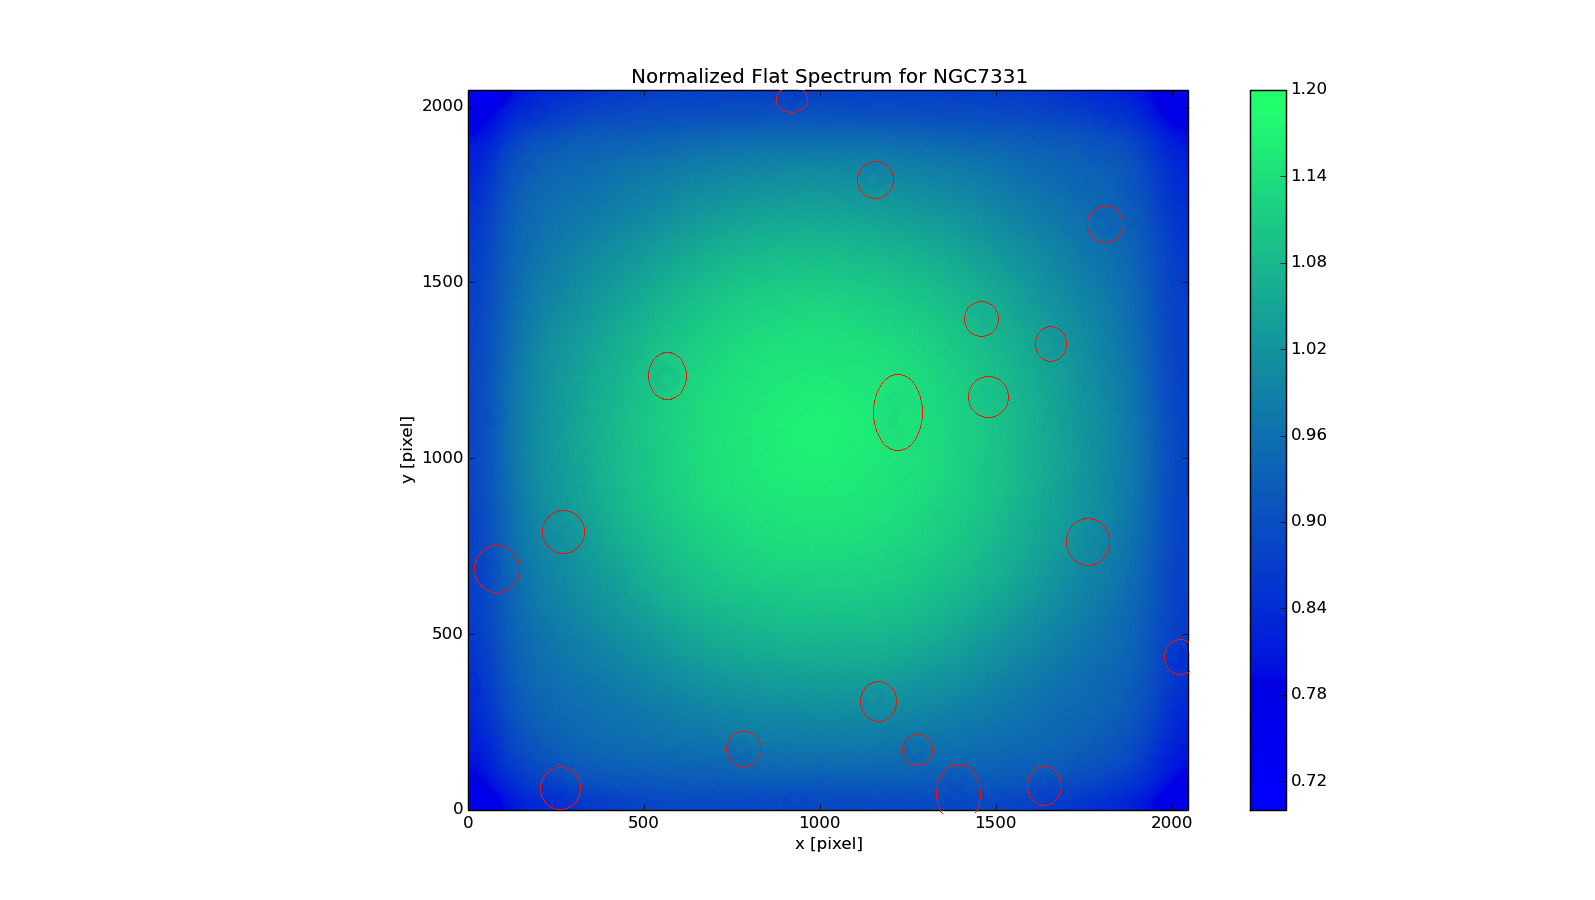
\includegraphics[width=\linewidth]{flatspectrum2.png}
  \caption{An example of a median-divided flat spectrum, this one used to reduce the NGC7331 image. The red circles mark torus anomalies.}
  \label{fig:flatspec}
\end{figure}

Another curious artifact was most obvious in the flat images. Cursory inspection of Figure~\ref{fig:flatspec} reveals that the CCD is apparently not uniformly illuminated in its twilight sky gazing. However, since stars are very nearly point sources, spanning only a few pixels, it is only the nearby pixel to pixel variation that will be of concern, rather than the overall trends. The latter would be significant only if relative intensity of the stars was a factor in the observations.

More difficult to spot were the strange torus-like anomalies in the image: donut-shaped areas with slightly lower intensity than the surrounding region. Several examples have been circled in Figure~\ref{fig:flatspec}. They are faint, but noticably features. However, close examination of the raw images showed that such toruses were present there as well. Data reduction was done as explained in Section~\ref{sec:data} in the hope that the location of these toruses was constant (some feature of the telescope's mirror perhaps), and would be accounted for by flat fielding.

%%%%%%%%%%%%%%%%%%%%%%%%%%%%%%%%%%%%%%%%%%

\section{Data Reduction and Methods}
\label{sec:data}

The first step towards analyzing the data was to reduce the noise and variations due to the camera itself. While the former, done by dark subtraction, is relatively trivial, the latter required some deliberation.

The flat file provided for the galaxy image had already been reduced, but the others required some modification. Flat fielding is meant to eliminate the pixel to pixel variations on a small scale, an example of which is shown in Figure~\ref{fig:flatzoom}.

\begin{figure}[!htbp]
  \centering
  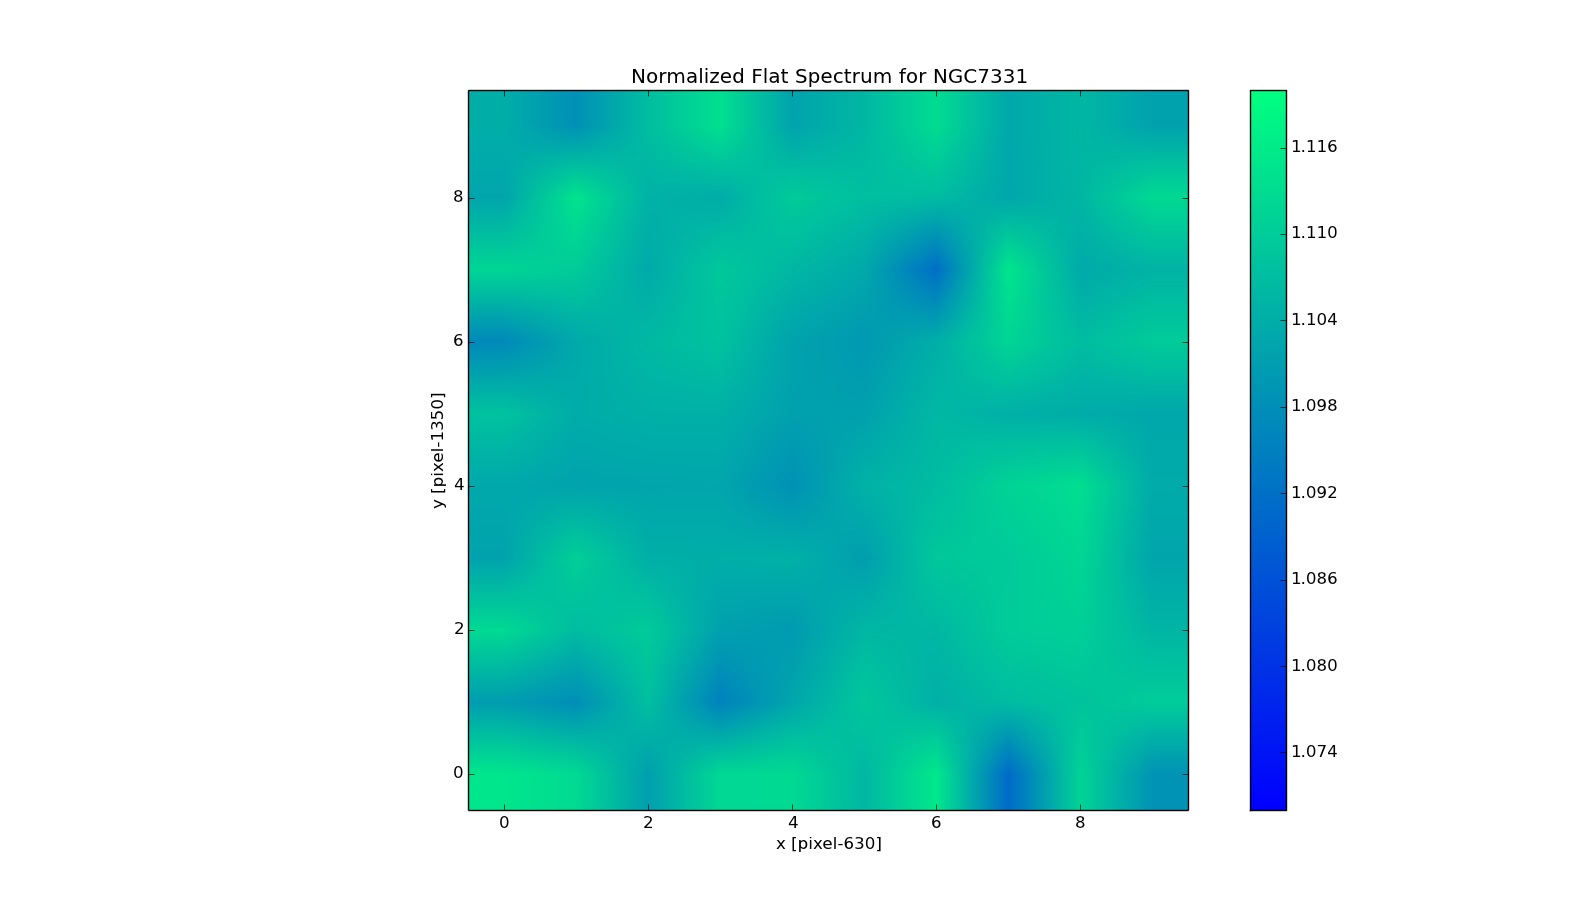
\includegraphics[width=\linewidth]{zoomflatspectrum.png}
  \caption{A zoomed-in section of the original flat in Figure~\ref{fig:flatspec}, showing pixel to pixel variations even in what appeared to be relatively uniform section (pixels (630,1350) to (640,1360)). Colourbar scale has been modified.}
  \label{fig:flatzoom}
\end{figure}

In order to get an accurate representation of the intesity variation between pixels without changing the raw data too much, the dark subtracted flat is divided by its median value. A formula for the ith pixel in the array is given by Equation~\ref{eqn:flat}, where $F_{pi}$ is the processed pixel, $F_{i}$ is the original flat pixel, $D_{i}$ is the dark pixel, and $m_{flat}$ is the median of the flat image.

\begin{equation}
F_{pi} = \frac{F_{i} - D_{i}}{m_{flat}}
\label{eqn:flat}
\end{equation}

With this normalized flat image, it is possible to process the raw spectrum. Equation~\ref{eqn:process} shows the calculation for the ith pixel in the array, where $P_{i}$ is the processed pixel, $R_{i}$ is the raw pixel, and $D_{i}$ and $F_{pi}$ retain their definitions from Equation~\ref{eqn:flat}.

\begin{equation}
P_{i} = \frac{R_{i} - D_{i}}{F_{pi}}
\label{eqn:process}
\end{equation}

Once the image had been processed through Python implementation of Equations~\ref{eqn:flat} and~\ref{eqn:process}, an image not unlike Figure~\ref{fig:galaxy} was produced. The next step was to identify the stars in the image. This was done by finding local maxima, using Python to check each pixel's intensity against its surroundings and threshold intensity. At each of these local maxima, Equation~\ref{eqn:centroid} was used to find the star's centroid, where i represents the number of the pixel being summed and ($\langle x \rangle$,$\langle y \rangle$) are the centroid's coordinates. The radius over which the sum was taken was limited to 25 pixels, and only pixels with intensity greater than the background limit were allowed to contribute.

\begin{equation}
\begin{array}{ccl}
\langle x \rangle &=& \sum_{i}x_{i}I_{i}/\sum_{i}I_{i}\\
\langle y \rangle &=& \sum_{i}y_{i}I_{i}/\sum_{i}I_{i}
\end{array}
\label{eqn:centroid}
\end{equation}

\begin{figure}[!htbp]
\centering
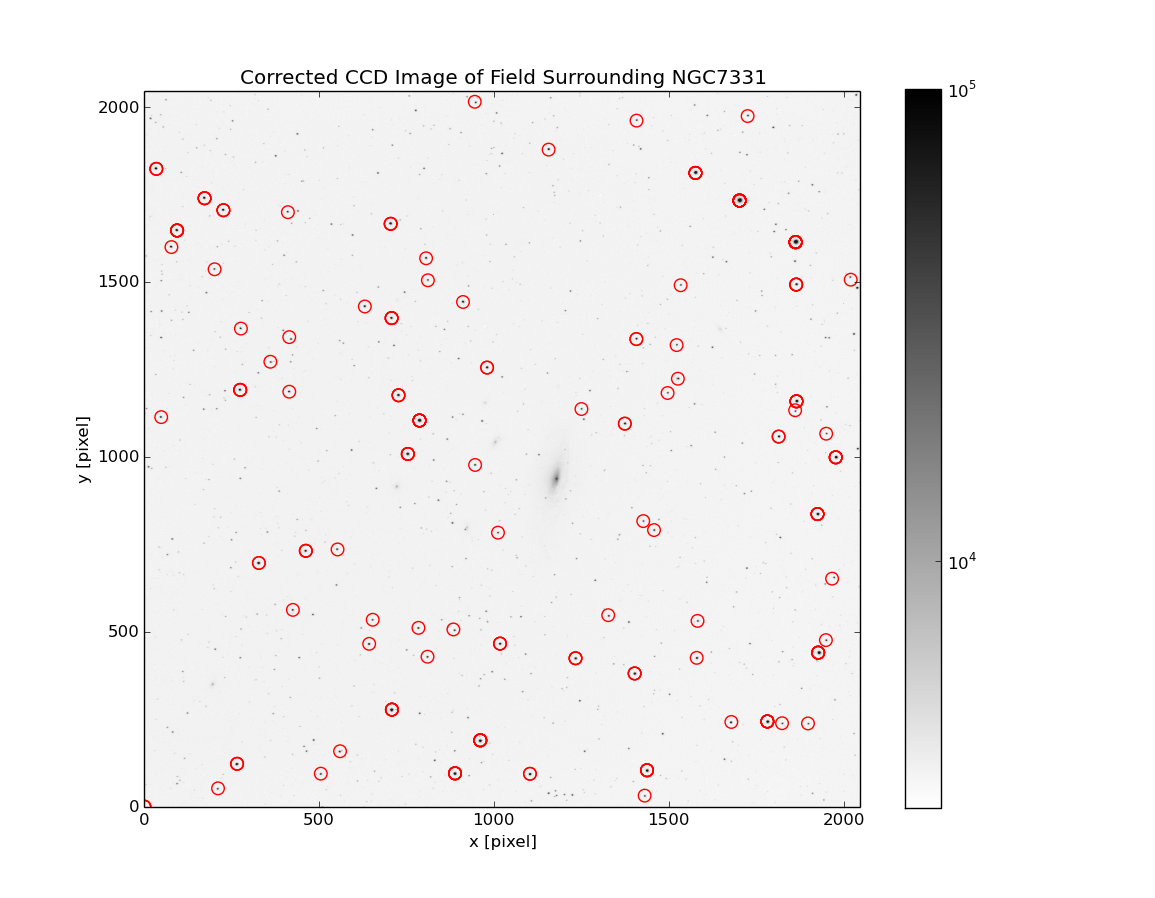
\includegraphics[width = \linewidth]{NGC7331.png}
\caption{Dark subtracted and flat field corrected galaxy image used to determine the plate constants. Intensity scale is logarithmic to make stars more immediately obvious. The red circles identify centroids found by the program.}
\label{fig:galaxy}
\end{figure}

With the centroids identified, the next step was to match up stars from the United States Naval Observatory (USNO) B1.0 Catalogue. Python code was provided to query the database, so all that remained was to set the field of view and transform the results into pixel locations.

Field of view was calculated as follows, using the provided telescope specifications from Section~\ref{sec:obs}.
\begin{center}
field of view = $fov = \frac{pixels}{(f/p)}$\\
$pixels = 2048$, $f = 3454$mm, $p = 0.018$mm\\
$\implies$ $fov = 0.011$ radians = $36.7'$
\end{center}

The resulting stars from the database were limited to magnitudes less than 13 and converted to standard coordinates ($X,Y$) with Equation~\ref{eqn:standard} implemented in Python. Following convention, $\alpha$ is right ascension, $\delta$ is declination and ($\alpha_{0},\delta_{0}$) are the equatorial coordinates of the center of the image. These coordinates were taken to be the right ascension and declination pointing of the telescope from the header file.

\begin{equation}
\begin{array}{ccl}
X &=& -\frac{cos\delta sin(\alpha-\alpha_{0})}{cos\delta_{0}cos\delta cos(\alpha-\alpha_{0})+sin\delta sin\delta_{0}}\\
Y &=& -\frac{sin\delta_{0}cos\delta cos(\alpha-\alpha_{0})-cos\delta_{0}sin\delta}{cos\delta_{0}cos\delta cos(\alpha-\alpha_{0})+sin\delta sin\delta_{0}}
\end{array}
\label{eqn:standard}
\end{equation}

These standard coordinates were then converted to pixel coordinates under the assumption that the CCD camera was an ideal one, using Equation~\ref{eqn:ideal}. This was not necessarily a reasonable assumption, but allowed the comparision of the centroids with the catalogue stars and the characterization of the nonideal camera (see Section~\ref{sec:calc}).

\begin{equation}
\begin{array}{ccl}
x &=& \frac{f}{p}X+x_{0}\\
y &=& \frac{f}{p}Y+y_{0}
\end{array}
\label{eqn:ideal}
\end{equation}

%%%%%%%%%%%%%%%%%%%%%%%%%%%%%%%%%%%%%%%%%%

\section{Calculations and Modelling}
\label{sec:calc}

Once the steps outlined in Section~\ref{sec:data} were carried out, it was possible to begin matching up stars from the catalogue and identified centroid locations. Even without camera corrections, there was a clear correlation between catalogue stars and the centroids (Figure~\ref{fig:catalogue}). A Python program was used to find the separation each centroid and each of the catalogue. The catalogue star that corresponded to the minimum separation was selected as matching the centroid. Some of the centroids remained unmatched, because the check for nearby catalogue stars was limited to a radius of 15 pixels.

\begin{figure}[!htbp]
\centering
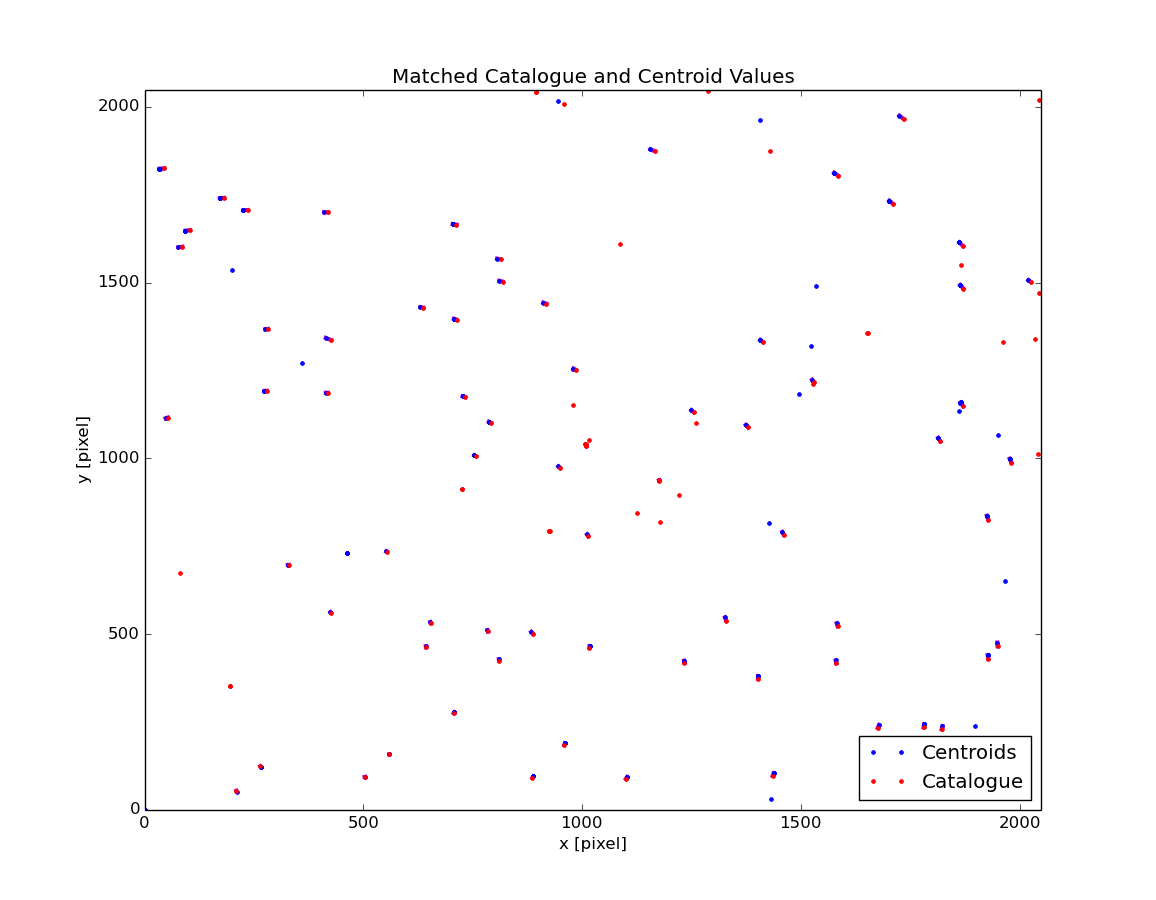
\includegraphics[scale=0.35]{first_match_galaxy.png}
\caption{Located centroids overplotted with catalogue stars of magnitude less than 13. The catalogue stars have been converted to pixels under the assumption that the camera is ideal.}
\label{fig:catalogue}
\end{figure}

The actual offsets between observed and predicted positions of the stars are shown in Figure~\ref{fig:separation} in terms of x and y pixel.

\begin{figure}[!htbp]
\centering
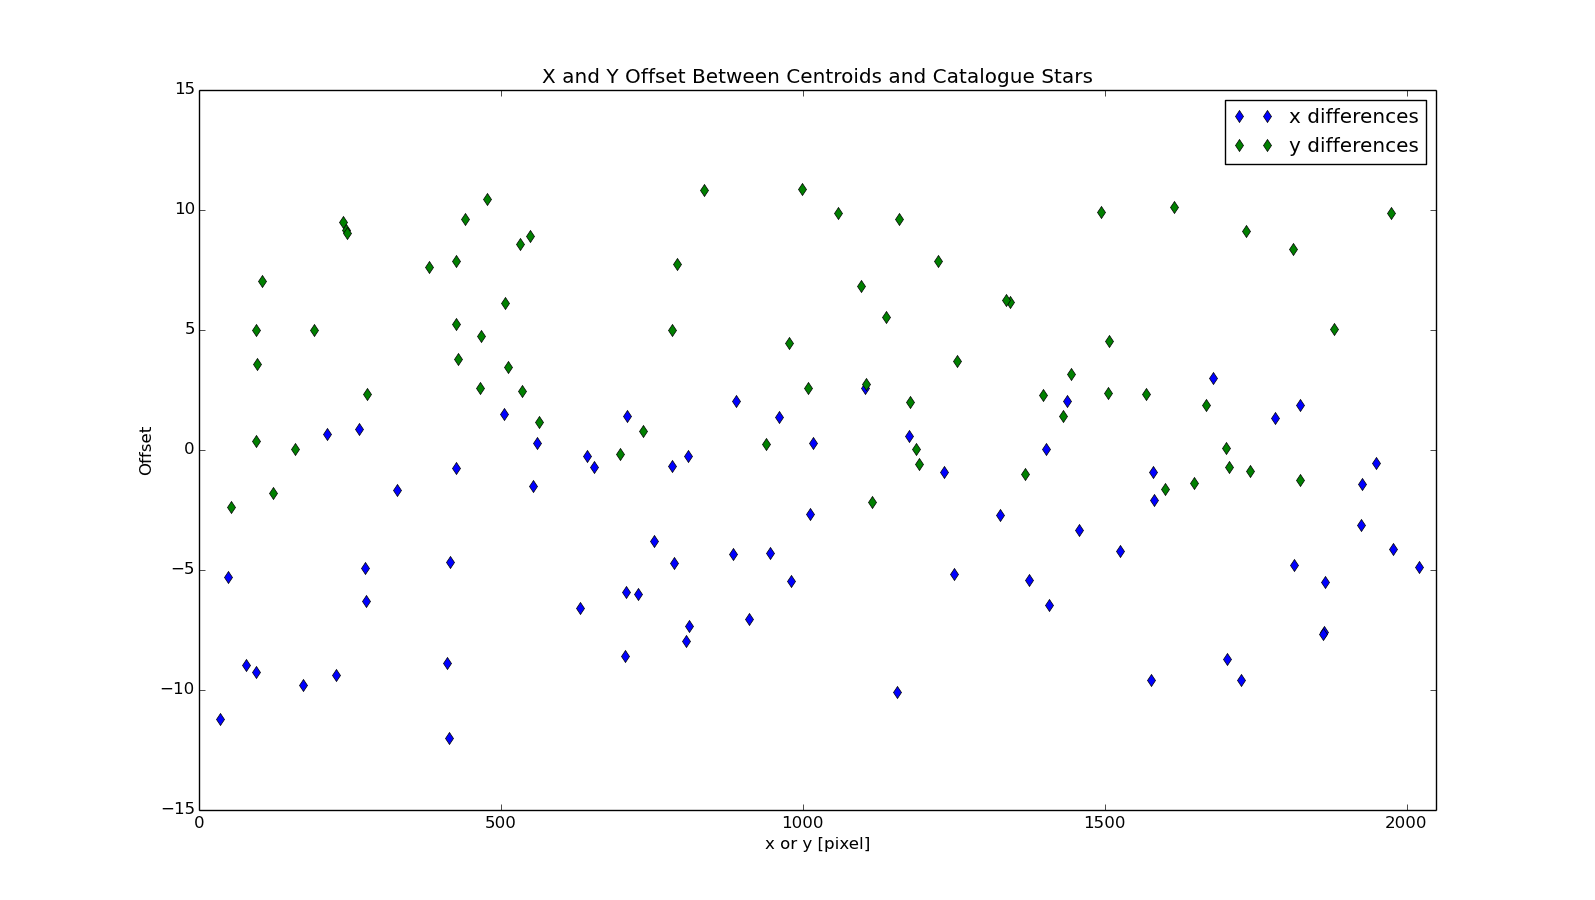
\includegraphics[scale=0.35]{separations.png}
\caption{Separations between matched catalogue stars and centroids in terms of number of x and y pixels.}
\label{fig:separation}
\end{figure}

These offsets made it clear that the assumption of an ideal camera was not the most appropriate one, and that there is some rotation between the two frames. To that end, new equations were considered to account for this possible rotation (Equation ~\ref{eqn:rotate}).

\begin{equation}
\begin{array}{ccl}
x &=& \frac{f}{p}(Xcos\theta - Ysin\theta)+x_{0}\\
y &=& \frac{f}{p}(Xsin\theta + Ycos\theta)+y_{0}
\end{array}
\label{eqn:rotate}
\end{equation}

It was simply a matter of calculating the angle $\theta$ of rotation, since $x,y$ were the pixel coordinates, $X,Y$ were the standard coordinates of catalogue and $x_{0},y_{0}$ the coordinates of the centre pixel. To this end, a matrix equation was set up for each matched pair of centroid ($\vec{x} = (x,y,1)$) and catalogue star ($\vec{X} = (X,Y,1)$), resulting in Equation~\ref{eqn:transform}.

\begin{eqnarray}
\mathbf{T} &=& \begin{pmatrix}
(f/p)a_{11}& (f/p)a_{12}& x_{0}\\
(f/p)a_{21}& (f/p)a_{22}& y_{0}\\
0& 0& 1
\end{pmatrix}\nonumber\\
\vec{x} &=& \mathbf{T}\vec{X}
\label{eqn:transform}
\end{eqnarray}

This equation required a bit of modification for Python implementation, namely, building separate matrices for the $x$ and $y$ pixel coordinates. The example for $x$ follows, where the matrices $\mathbf{a}$ and $\mathbf{B}$ are defined by showing their ith row, since each row will have the same structure.

\begin{center}

$\mathbf{a} = \mathbf{B}\mathbf{c}$\\

$\mathbf{a}_{i} = x_{i}$, $\mathbf{B}_{i}$ = ($(f/p)X_{i}$  $(f/p)Y_{i}$   $1$) and $\mathbf{c}$ = ($a_{11}$  $a_{12}$  $x_{0}$)\\

\begin{equation}
\mathbf{c} = (\mathbf{B}^{T}\mathbf{B})^{-1}\mathbf{B}^{T}\mathbf{a}
\label{eqn:constants}
\end{equation}

\end{center}

Using Equation~\ref{eqn:constants}, it was possible to determine the transformation constants for $x$. Similar steps were carried out for the $y$ coordinate, with the results shown in Table~\ref{tab:constants}.

\begin{center}
\begin{table}[!htbp]
  \centering
  \begin{tabular}{c||c||c}
  	Constant & Ideal Value & Calculated Value \\
  	\hline
  	\hline
  	$a_{11}$ & 1 & 1.00050002 \\
  	$a_{12}$ & 0 & -0.00659824 \\
  	$x_{0}$ & 1024 & 1019.64337372 \\
  	$a_{21}$ & 0 & 0.00626632 \\
  	$a_{22}$ & 1 & 0.99983162 \\
  	$y_{0}$ & 1024 & 1028.3480059 \\
   \end{tabular}
    \caption{A comparison of constant values for an ideal camera (Equation~\ref{eqn:ideal}) and those fitted to the centroids.}
    \label{tab:constants}
\end{table}
\end{center}

Applying the constants to the transformation of the catalogue stars to pixel coordinates resulted in a much closer match (Figure~\ref{fig:residuals}). The residuals were averaged and the result of each average was taken to be the uncertainty in the pixel locations. This was a sensible measure of error because it quantifies the difference between the transformed location and the observed position. This resulted in $\Delta x$ = 0.755 pixels, $\Delta y$ = 0.756 pixels.

\begin{figure}[!htbp]
\centering
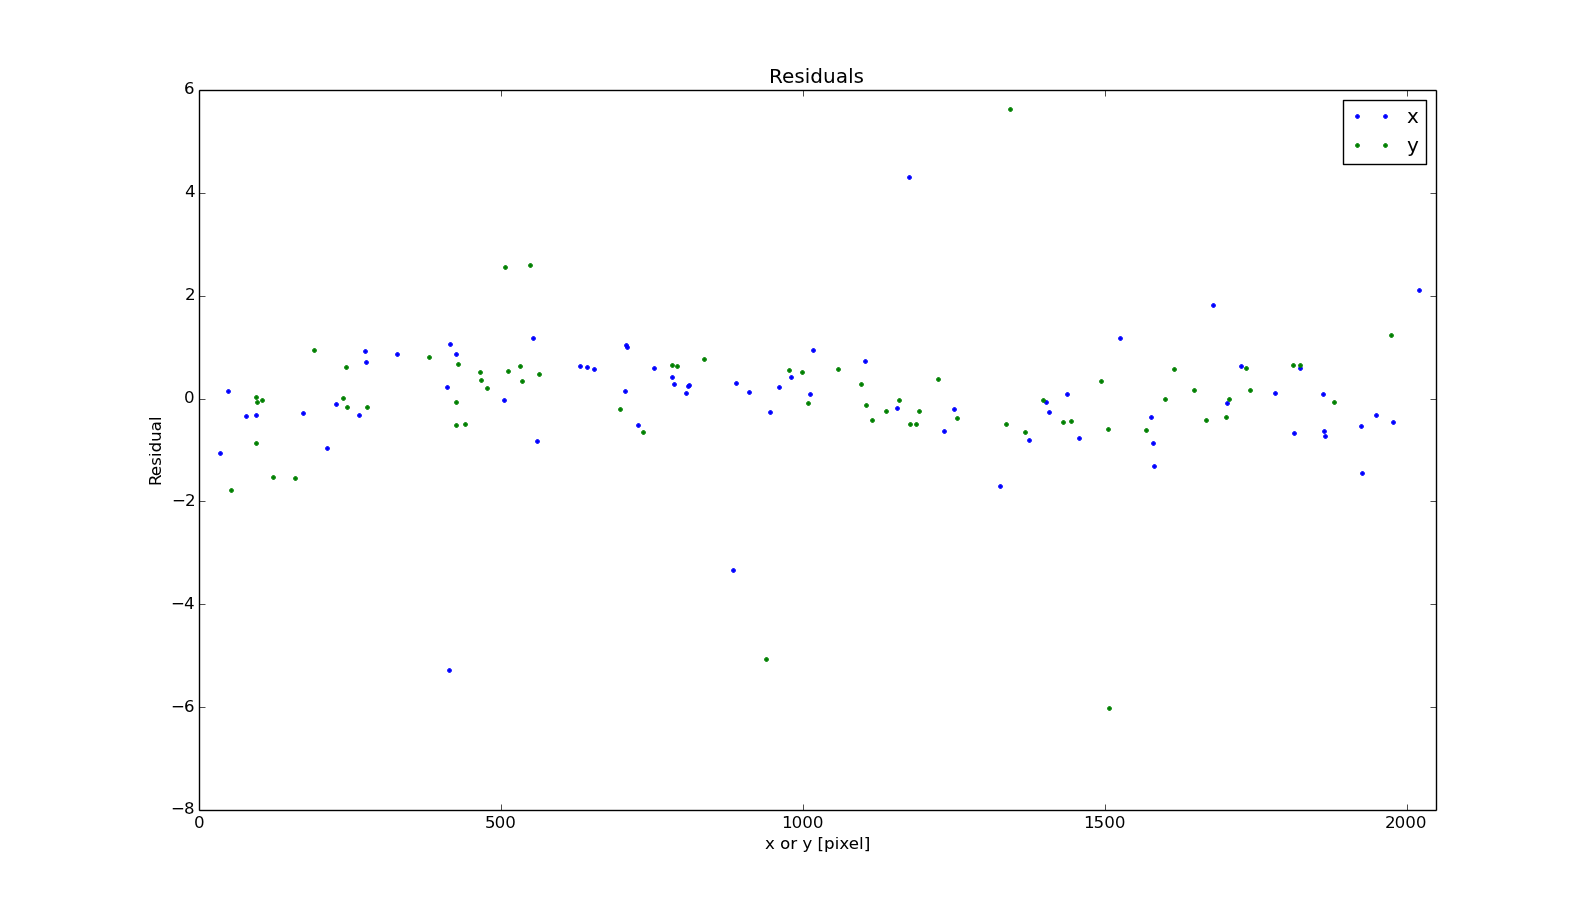
\includegraphics[scale = 0.35]{fit_residuals.png}
\caption{Residuals in x and y pixel between the centroids and the catalogue stars with new transformation parameters}
\label{fig:residuals}
\end{figure}

\begin{equation}
\chi ^{2}_{reduced} = (\mathbf{a}-\mathbf{B}\mathbf{c})^{T}(\mathbf{a}-\mathbf{B}\mathbf{c})
\label{eqn:chi}
\end{equation}

In spite of few outliers, the residuals of this fit were centered around zero in both $x$ and $y$ (Figure~\ref{fig:residuals}). The goodness of the fit could be quantified using Equation~\ref{eqn:chi} for $\chi^{2}_{reduced}$. It was found that $\chi^{2}_{reducedx}$ = 1.43784932, while $\chi^{2}_{reducedy}$ = 1.98449692.

Given these new transformation constants, and assuming that they would not change in the three month period separating the galaxy observations and those of the asteroid, analysis of the images of 30 Urania began. The raw images were reduced and centroids were located as outlined in Section~\ref{sec:data}. The resulting images are shown in Figure~\ref{fig:urania}

\begin{figure}[!htbp]
\centering
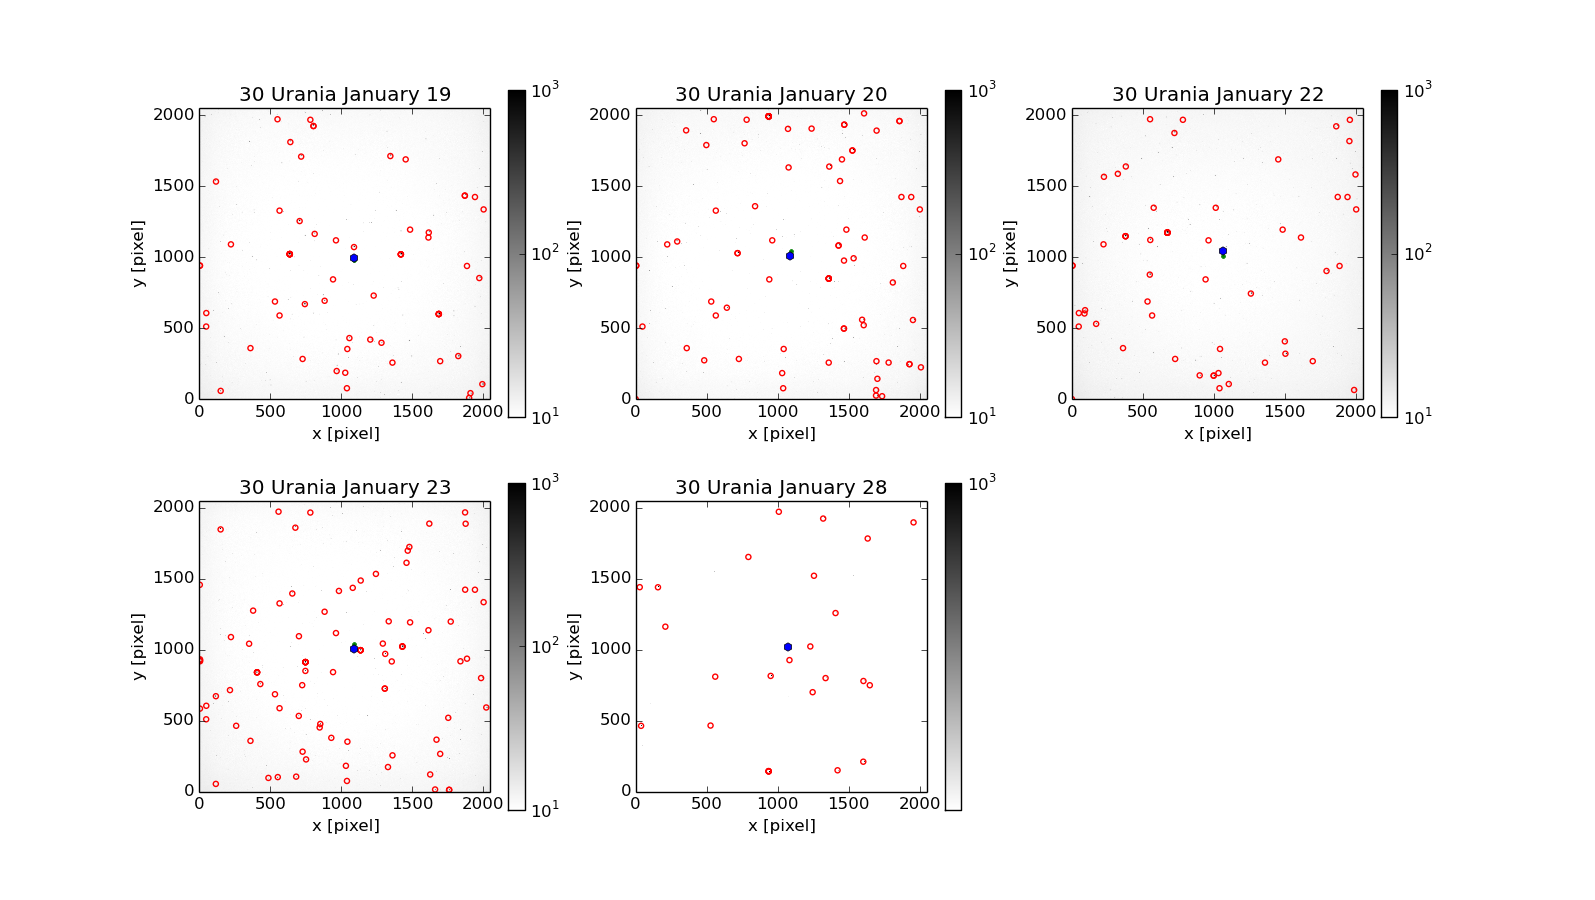
\includegraphics[width = \linewidth]{urania_centroid_fix2.png}
\caption{Star centroids for the five days of observations of 30 Urania. The green marker represents the apparent position of the asteroid, the blue marker the nearest centroid.}
\label{fig:urania}
\end{figure}

The asteroid was identified in the reduced flats using SAOImage DS9. Since the telescope would have been focussed with the asteroid somewhere near the centre of the image, it was simply a matter of identifying patterns of stars common to subsequent images and finding the point that did not match. Being relatively nearby, the asteroid was quite bright, and once a pattern was identified, its presence was obvious. This strategy worked well for the first four days of observations, but broke down on the final one, because there was no overlap of stars to be used for comparison. In this final image, the asteroid was identified by educated guess.

Once the asteroid's approximate position had been determined, its actual location was found by finding the closest centroid identified in the image using a variation of the Python code used to match up catalogue stars and centroids. Once these points were found, they were transformed to equatorial coordinates. First, the inverse of Equation~\ref{eqn:transform} was applied, using the derived plate constants. This transformed the pixel locations to standard coordinates. These standard coordinates were then transformed to right ascension and declination using Equation~\ref{eqn:radec}.

\begin{equation}
\begin{array}{ccl}
\alpha &=& tan^{-1}\left(-\frac{X}{cos\delta_{0}-Ysin\delta_{0}}\right) + \alpha_{0}\\
\delta &=& sin^{-1}\left(\frac{sin\delta_{0} + Ycos\delta_{0}}{\sqrt{1+X^{2}+Y^{2}}}\right)
\end{array}
\label{eqn:radec}
\end{equation}

Once the coordinates had been transformed to the equatorial system, the points were plotted against time and a line of best fit was found using the the scipy.optimize.leastsq module (Figure~\ref{fig:pm}). The errors in x and y were also transformed, to give position uncertainty of $\Delta\alpha = 0.890''$, $\Delta\delta = 0.817''$.

\begin{figure}[!htbp]
\centering
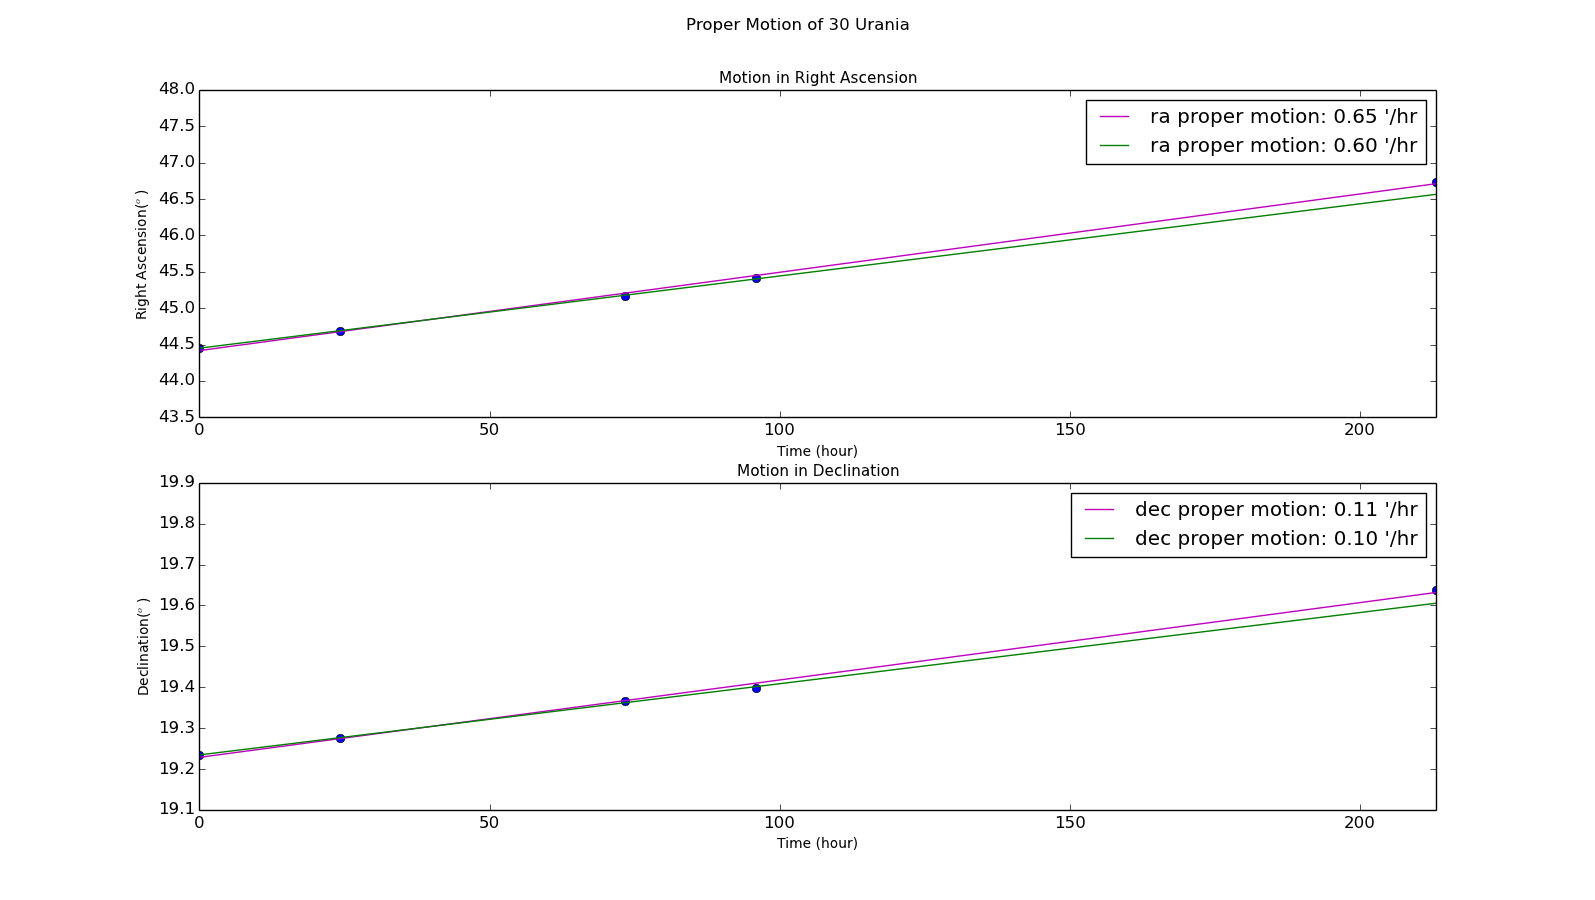
\includegraphics[scale = 0.35]{proper_motion.png}
\caption{Motion in right ascension and declination of 30 Urania over observing time. Error bars are plotted, but are hidden by the markers.}
\label{fig:pm}
\end{figure}

Two fits were made, one to the first four points, and another including the last point (about which there was less certainty). The resulting proper motions are listed in Table~\ref{tab:pm}. The uncertainty was found by averaging the residuals between the fitted proper motion and the individual proper motion calculated between consecutive points.

\begin{center}
\begin{table}[!htbp]
  \centering
  \begin{tabular}{c||c||c||c||c}
  	Points & $\mu_{\alpha} (^o/hr)$ & $\mu_{\alpha} (''/hr)$ & $\mu_{\delta} (^o/hr)$ & $\mu_{\delta} (''/hr)$ \\
  	\hline
  	\hline
  	4 & $9.93\e{-3}\pm 4\e{-5}$ & $35.7\pm 0.2$ & $1.74\e{-3}\pm 6\e{-5}$& $6.3\pm 0.2$ \\
  	5 & $1.08\e{-2}\pm 8\e{-4}$ & $39\pm 2$ & $1.9\e{-3}\pm 2\e{-4}$ & $6.8\pm 0.8$ \\
   \end{tabular}
    \caption{Comparison of proper motion when making a linear fit of the position of the asteroid. The first row considers only the first four points (green fit line in Figure~\ref{fig:pm}), about which there is more certainty. The second row includes the final point as well (pink fit line in Figure~\ref{fig:pm}).}
    \label{tab:pm}
\end{table}
\end{center}



%%%%%%%%%%%%%%%%%%%%%%%%%%%%%%%%%%%%%%%%%%

\section{Discussion}
\label{sec:discussion}

The final result of all of the calculations is illustrated in Figure~\ref{fig:path}. The figure shows a tangent plane approximation of the sky (the sphere plotted in two dimensions). The asteroid position has been marked, and a line showing its proper motion across the sky drawn through the star field of centroids.

\begin{figure}[!htbp]
\centering
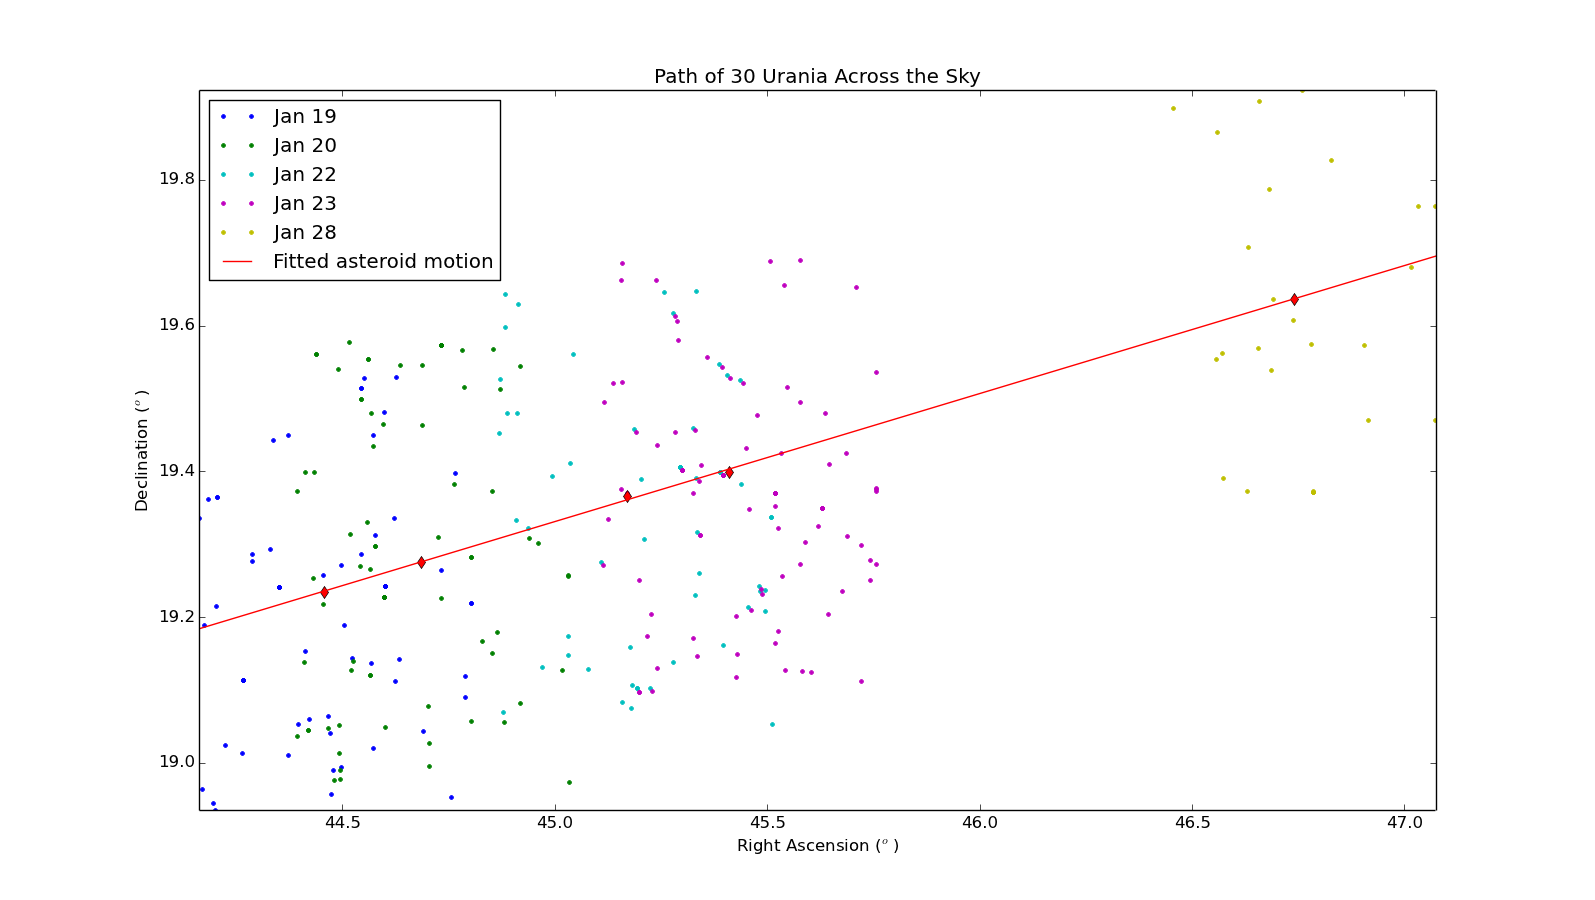
\includegraphics[width = \linewidth]{path_urania.png}
\caption{Path of 30 Urania across the sky. Centroids are also plotted, for reference.}
\label{fig:path}
\end{figure}

One feature that can be immediately noted about Figure~\ref{fig:path} is the constant offset of the background stars. The first four days of observations covered overlapping portions of the sky (this fact was used in locating the asteroid itself). Thus in the image, there are stars from different days that correspond to each other. This is easiest to see in the comparison of the January 22 and January 23 data, where the stars overlap. However, it is clear that there is a constant offset between the star patterns for the earlier two days. Unlike the plots where database stars were compared to centroids, the shift between the two sets is constant, but different for each pair.

Since each day's pixel coordinates goes through the same transformation to equatorial coordinates (using the same plate constants), there are two possible reasons for this strange offset. The first is that the plate constants since the previous October for which they were calculated (Table~\ref{tab:datatable}). However, this would imply that the plate constants vary rather exteremely from day to day. The other possiblility is that the $\alpha_{0}$ and $\delta_{0}$ used in Equation~\ref{eqn:radec} were not the actual coordinates upon which the telescope was centered. The $\alpha_{0}$ and $\delta_{0}$ were taken from the fit file, and while those coordinates are where the telescope believed it was pointing, poor calibration or some other pointing error would mean that those coordinates were not correct.

As a further check of the asteroid coordinates, NASA's Jet Propulsion Laboratory HORIZON's database~\citep{urania} was queried to get an ephemeris for 30 Urania over the relevant dates. Table~\ref{tab:position} shows the results of that ephemeris for the times specified in the fits files compared with the asteroid's position in the data.

\begin{center}
\begin{table}[!htbp]
  \centering
  \begin{tabular}{c||c||c||c||c||c||c}
  	Day & Identified $\alpha$ & Ephemeris $\alpha$ & Offset (s) & Identified $\delta$ & Ephemeris $\delta$ & Offset ($''$)\\
  	\hline
  	\hline
  	Jan 20 & 02:57:49.44 & 02:57:49.26 & 0.18 & +19:14:02.7 & +19:14:30.8 & 28.1\\
  	\hline
  	Jan 21 & 02:58:44.30 & 02:58:44.11 & 0.19 & +19:16:34.8 & +19:16:45.1 & -10.3\\
  	\hline
  	Jan 23 & 03:00:40.71 & 03:00:40.75 & 0.04 & +19:21:57.4 & +19:21:38.2 & 19.2\\
  	\hline
  	Jan 24 & 03:01:38.39 & 03:01:37.59 & 0.80 & +19:23:56.0 & +19:24:04.0 & -8.0\\
  	\hline
  	Jan 25 & 03:06:57.74 & 03:02:30.46 & 267 & +19:38:12.9 & +19:26:21.6 & 711
   \end{tabular}
    \caption{A comparison of asteroid position as identified within the program and asteroid position according the JPL's ephemeris~\citep{urania}. Dates are all from 2012. By convention, right ascension ($\alpha$) is given in hours, and declination ($\delta$) is given in degrees.}
    \label{tab:position}
\end{table}
\end{center}

It is obvious from the Table~\ref{tab:position} that for the first four days, the asteroid's position matches the predicted position quite well. However, on the last day, it is clear that the asteroid was completely misidentified. Therefore, final values for proper motion are taken from the fit of the first four points. Both fits were plotted on Figure~\ref{fig:path}, but the scaling is such that they are completely indistinguishable.

The offsets in Table~\ref{tab:position} are outside the errors calculated in Section~\ref{sec:calc}, where it was found that $\Delta\alpha = 0.890''$ and $\Delta\delta = 0.817''$. This is not entirely unexpected. The ephemeris could only be generated for thirty minute intervals (as any longer time crashed the webpage), and so the observation times had to be rounded to the nearest half hour. For a slow moving star, this would not be a problem, but in the case of 30 Urania, Table~\ref{tab:pm} clearly shows that a large shift in arcseconds should be expected even over a short time. While some shift was expected, the January 25 asteroid location is still well outside the expected value.

With this external assessment of the points used, the proper motion was taken from the fit of the first four points, namely that $\mu_{\alpha} = 35.7\pm 0.2 ''/hr$ and $\mu_{\delta} = 6.3\pm 0.2 ''/hr$.

\bibliographystyle{plainnat}
\bibliography{cite}

\end{document}